\documentclass[12pt]{article}
\usepackage{geometry}
\geometry{left=1in,right=0.75in,top=1in,bottom=1in}

%%%%%%%%%%%%%%%%%%%%%%%%%%%%%%%%%%%%%%%%
% Replace ABCDEF in the next line with your chosen problem
% and replace 1111111 with your Team Control Number
\newcommand{\Problem}{E}
\newcommand{\Team}{2102362}
%%%%%%%%%%%%%%%%%%%%%%%%%%%%%%%%%%%%%%%%

\usepackage{newtxtext}
\usepackage{amsmath,amssymb,amsthm}
\usepackage{indentfirst}
\usepackage{gensymb}
\usepackage{setspace}
\usepackage{subfigure}
\usepackage{listings}
\usepackage{bm}
\usepackage{float}
\usepackage{newtxmath} % must come after amsXXX
\usepackage{textcomp}
\usepackage{graphicx}
\usepackage{cite}
\usepackage{xcolor}
\usepackage{fancyhdr}
\usepackage{booktabs}
\usepackage{multirow}
\usepackage{makecell}
\usepackage{epstopdf}
\usepackage{hyperref}
\usepackage{titlesec}
\usepackage{titletoc}
\usepackage{appendix}
\usepackage{url}
\usepackage[final]{pdfpages}
\linespread{1}
\setlength{\parskip}{0.5\baselineskip}
\setlength{\parindent}{2em}
\lhead{Team \Team}
\rhead{}
\cfoot{}

\newtheorem{theorem}{Theorem}
\newtheorem{corollary}[theorem]{Corollary}
\newtheorem{lemma}[theorem]{Lemma}
\newtheorem{definition}{Definition}

%%%%%%%%%%%%%%%%%%%%%%%%%%%%%%%%
\setlength{\headheight}{15pt}

\begin{document}
\graphicspath{{.}}  % Place your graphic files in the same directory as your main document
\DeclareGraphicsExtensions{.pdf, .jpg, .tif, .png}
\thispagestyle{empty}
\vspace*{-16ex}
\centerline{\begin{tabular}{*3{c}}
        \parbox[t]{0.3\linewidth}{\begin{center}\textbf{Problem Chosen}\\ \Large \textcolor{black}{\Problem}\end{center}}
         & \parbox[t]{0.3\linewidth}{\begin{center}\textbf{2021\\ MCM/ICM\\ Summary Sheet}\end{center}}
         & \parbox[t]{0.3\linewidth}{\begin{center}\textbf{Team Control Number}\\ \Large \textcolor{black}{\Team}\end{center}} \\
        \hline
    \end{tabular}}
%%%%%%%%%%% Begin Summary %%%%%%%%%%%

\begin{center}
    {\Large \quad Prior Factors of a Food System: Money or Balance? \newline Case Studies on China, USA, and Ethiopia }

    \vspace{1em}
    {\large \textbf{Summary}}
\end{center}
\vspace{-0.5em}

\textbf{Food system} is an integrated concept reflecting human activities in the production and acquisition of food. A food system is strongly associated with other systems such as economy system, ecology system, and society system. Nowadays, the stability of a food system are of greater and greater significance for building a harmonious society and promoting national development. However, at present our global food system works mainly based on the control of market, where people in the system are blindly in pursuit of high efficiency and high profitability, causing problems including the imbalance of distribution and environmental degradation. The aim of this report is to \textbf{build a re-optimization model} to evaluate the result of reordering the significance of different \textbf{indicators}. These indicators are efficiency, profitability, equity, and sustainability. We also establish a \textbf{predictive model} to reflect the change of the food system along with time variation. Besides, we do case studies and discuss the completeness of the model. 

For the re-optimization model, we collect data of 18 indices in 3 countries from 2000 to 2020 in total, and use these indices to build four models for the four indicators. In this part, we first adopt the \textbf{logistic model} to predict the population change. Then we build an differential equation for finding efficiency, and use \textbf{Runge-Kutta method} to get the numerical solution. According to the results, we build a model for evaluating equity. Next, in the model for evaluating profitability, we use \textbf{linear programming} to ensure that the data we use is within a reasonable range. Finally, we use \textbf{linear} and \textbf{nonlinear fitting} method to evaluate sustainability. 

For the prediction model, we normalize all the data we derived, and then obtain the values of weight through \textbf{analytic hierarchy process (AHP)}. We assess the validity of the weights to prove the correctness of comparison matrix. We also provide calculations of the final prioritized food system index $PFSI$ by doing a special \textbf{weighted summation}. The result of $PFSI$ shows the food system evaluation results under a certain degree of emphasis for the four indicators. If $PFSI$ is closer to 0, then the focus of the food system we analyze is more on efficiency and profitability. If the result is closer to 0, then the focus is more on sustainability and equity.

For the discussion section, we first use the data we collected for the prediction of the food system after re-optimization. Then, we discuss the benefits and costs for changing the order of the four indicators. We apply our model into \textbf{China}, \textbf{USA}, and \textbf{Ethiopia} for case studies and analyze the different consequence between developing countries and developed countries. Moreover, we pay attention to the scalability and adaptability of the model. Finally, we discuss the strengths and potential improvements of the food system model.



\vspace{2em}
\textbf{Keywords}: Food system, Analytic hierarchy process (AHP), Logistic model, Linear Programming, Runge-Kutta method, Nonlinear fitting, Linear fitting

% to here
%%%%%%%%%%% End Summary %%%%%%%%%%%

%%%%%%%%%%%%%%%%%%%%%%%%%%%%%%
\clearpage
\pagestyle{fancy}
% Uncomment the next line to generate a Table of Contents

\newpage
\setcounter{page}{1}
\rhead{Page \thepage\ }
%%%%%%%%%%%%%%%%%%%%%%%%%%%%%

\titlecontents{section}[0cm]{\fontsize{12pt}{\baselineskip}\selectfont}{\hspace*{3em}\contentslabel{2em}\ }%
{}{\titlerule*[0.5pc]{$\cdot$}\contentspage\hspace*{1cm}\vspace*{-0.3em}}%

\titlecontents{subsection}[1cm]{\fontsize{10pt}{\baselineskip}\selectfont}{\hspace*{3em}\contentslabel{2em}\ }%
{}{\titlerule*[0.5pc]{$\cdot$}\contentspage\hspace*{1cm}\vspace*{-0.5em}}%

\titlecontents{subsubsection}[2cm]{\fontsize{10pt}{\baselineskip}\selectfont}{\hspace*{3em}\contentslabel{2em}\ }%
{}{\titlerule*[0.5pc]{$\cdot$}\contentspage\hspace*{1cm}\vspace*{-0.6em}}%

\tableofcontents


\newpage
%%%%%%%%%%%%%%%%%%%%%%%%%%%%%
\section{Introduction}
\vspace{-1em}
\subsection{Background}


The food system is conceived as a set of human activities from food production to processing, distribution, and consumption \cite{cite:Prior}. Its complexity shows up in its manifold drivers, feedback, outcomes, and relations with other human systems, and its concepts are constantly enriched with human's increasing attention to its connotation. From a macroscopic perspective, the current analysis of food systems is strongly connected to the topic of \textbf{food security}, which refers to a goal that everyone in the world can get access to sufficient and nutritious food to satisfy the diet needs \cite{cite:Concept}. For example, a scientific group for the 2021 United Nations food systems summit suggests that the ability of the food system to enable every human to be well-nourished should be the core of the overall action tracks, which can be recognized as a pursuit for sustainability and equity \cite{cite:Summit}.

\vspace{-1em}
\begin{figure}[H]
    \centering
    \includegraphics[width = 0.5\textwidth]{figure/FS.pdf}
    \vspace{-1em}
    \caption {Sustainable food systems \cite{cite:fig}}
\end{figure}

\vspace{-1em}
However, due to the leading rule of the market, at present the prior objective of the global food system is maximum efficiency along with the highest profit \cite{cite:Market}. The market control of trade and prices and regional inherent inequities make the basic demands for food by many kinds of vulnerable groups hard to be satisfied. As a result, distribution problems such as food waste and food shortage have emerged. For example, in 2016 about 10.7\% people in the world suffer from malnutrition problems, but at the same time about 1/3 of all the food produced is wasted \cite{cite:USDA}. Furthermore, negative interactions that are exerted between the food system and other correlated systems like environment system and economic system make the dilemma of the food system harder to solve. 

\vspace{-1em}
%%%%%%%%%%%%%%%%%%%%%%%%%%%%%
\subsection{Restatement of the Problem}

To ensure a more stable food system with a more comprehensive selection of different objectives, an optimization model must be established to improve the current conditions of the food system. As a consultant team for the International Comestibles Management (ICM) Committee, we are going to implement the following tasks:

\begin{itemize}
    \item Find the factors related to the food system, determine the objectives of our model, and choose representative indicators.
    \item According to the indicators we fix, build a comprehensive evaluation model for the current food system.
    \item Re-optimize the food system given a more preferable objective, and compare the ideal food system with the current one, and then analyze the feasibility of improving the food system.
    \item Discuss the trade-offs of optimization, including both benefits and costs of the change.
    \item Apply the model to countries with different levels of development and compare the results.
    \item Analyze the extendability and adaptability of the food system model. 
\end{itemize}

\vspace{-1em}
%%%%%%%%%%%%%%%%%%%%%%%%%%%%%
\subsection{Our Work}
Our efforts can be summarized in the following flow chart.
\begin{figure}[H]
    \centering
    \includegraphics[width = 1\textwidth]{figure/procedure.pdf}
    \caption{Structure of the model and paper}
    \label{procedure}
\end{figure}

\section{Assumptions and Justifications}

We make the following assumptions in the modelling process. 

\noindent \textbf{Assumption 1.} \textit{Country is the unit of a food system.}

According to the instructions of the question of comparison between developed and developing countries, we assume that our evaluation for food systems is conducted in terms of country, and the model only synthesizes the consideration of food system for profitability, efficiency, equity, and sustainability.

\noindent \textbf{Assumption 2.} \textit{Imports and exports among countries are neglected.}

We assume that we do not consider the import and export of food among countries. In addition, we assume that food is distributed equally within the country we study. Since based on the data provided by FAO almost all the major countries in the world have the self-sufficiency rate of food larger than 0.8 \cite{cite:Self_support}, we regard each country we analyze as an independent place where people produce and market all by themselves. 

\noindent \textbf{Assumption 3.} \textit{All the data is reliable and precise.}

We assume that the data we collected from databases are reliable. They are from major websites including FAO \cite{cite:FAO_data}, World bank \cite{cite:Worldbank}, Statista \cite{cite:Statista}, and Worldometers \cite{cite:Worldometers}.

\noindent \textbf{Assumption 4.} \textit{Unpredictable natural disasters and other sudden changes will not happen.}

Unforeseen natural hazard such as drought and flood disasters will affect the food system as well as its indices dramatically, so we assume that within the predicted time there are no sudden far-reaching changes.

\noindent \textbf{Assumption 5.} \textit{The change in the population of a country is continuous.}

Since indices of the model is based on the population in a country, we assume that there are not mass migrations or wars that could affect the population in the country. 

%%%%%%%%%%%%%%%%%%%%%%%%%%%%%
\section{Model Preparation}
\subsection{Notation}

In this paper, we define some symbols and parameters, and their notations are shown in Table \ref{tab:notation}.


\begin{table}[!h]
    \centering
    \caption{\label{tab:notation} Notations}
    \vspace{1em}
    \begin{tabular}{lll}
        \toprule
        Symbols & Description & Units \\
        \midrule
        $t$ & time & year \\
        $PM$ & Policy motivation, an adjustable constant & 1 \\
        $UR_{2020}$ & Undernourishment rate in 2020 & \% \\
        $OR_{2020}$ & Obesity rate in 2020 & \% \\
        $p(t)$ & Population & person\\
        $p_{2020}$ & Population in 2020 & person \\
        $S_m(t)$ & Target total yield in year $t$ & ton \\
        $S(t)$ & Total yield & ton \\
        $S_{2020}$ & Total yield in 2020 & ton \\
        $s_1(t)$ &Target total yield of cereal in year $t$& ton\\
        $s_2(t)$ &Target total yield of fruit in year $t$& ton\\
        $s_3(t)$ &Target total yield of oil crops in year $t$& ton\\
        $s_4(t)$ &Target total yield of vegetables in year $t$& ton\\
        $s_5(t)$ &Target total yield of dairy in year $t$& ton\\
        $s_6(t)$ &Target total yield of meat in year $t$& ton \\
        $PR_i(t)$ &The corresponding average prices for six different foods in year $t$ & \$/ton \\
        $IF$ &Average inflation rate of the studied country from 2000 to 2020 & \%\\
        $IN(t)$ &The annual income of the Food sales in year $t$ & 100000 \$ \\
        $GHG(t)$ & Total greenhouse gas emissions from agriculture in year $t$ & CO$_2$ equivalent \\
        $r_1$ & Weight of efficiency & 1 \\
        $r_2$ & Weight of equity & 1 \\
        $r_3$ & Weight of profitability & 1 \\
        $r_4$ & Weight of sustainability & 1 \\
        $rs$  & Relative significance of \textit{EQ} (or \textit{SU}) with respect to \textit{EF} (or \textit{PF}) & 1\\
        $EF(t)$ & Score of efficiency in the food system & 1 \\
        $EQ(t)$ & Score of equity in the food system & 1 \\
        $PF(t)$ & Score of profitability in the food system & 1 \\
        $SU(t)$ & Score of sustainability in the food system & 1 \\
        $PFSI(t)$ & Prioritized food system index & 1 \\
        \bottomrule
    \end{tabular}
\end{table}


%%%%%%%%%%%%%%%%%%%%%%%%%%%%%
\section{Model Design}

To complete our model for the food system, we use $EF$, $EQ$, $PR$, and $SU$ to denote the score of efficiency, score of equity, score of profitability, and score of sustainability respectively. Then the final food system index $PFSI$ can be derived by a special weighted average process. 

\subsection{Preparation: Classic Population Logistic Prediction Model}

To predict the population in the future for each year, we searched for possible population forecasting models in the database. We choose \textbf{logistic model} to complete the prediction \cite{cite:logi}, since compared with \textbf{Malthus model} we should consider constraints on natural resources, environmental capacity and policies to give a changing population growth rate $r$. We use \textbf{linear least square method} to obtain the initial value $r_0$ and maximum population $P_{max}$. The solution procedure is shown below.

\begin{enumerate}
    \item Collect population data of China, USA, and Ethiopia from 2000 to 2020.
    \item Suppose the population growth rate $r$ is a function varying with population $P$: $r(P) = r_0 - P$. The equation of the logistic model is given by $$\frac{\mathrm{d} P}{\mathrm{d} t} = r_0 (1-\frac{P(t)}{P_{max}})P(t).$$
    \item Get the difference equation by backward difference:
    
    $$\frac{P(k)-P(k-1)}{P(k)} = r_0 - s\cdot P(k),\text{ }k = 2, 3, \cdots, 21.$$
    
    \item Fit the parameters $r_0$ and $P_{max}$ by linear least square method. The result of China and USA are shown in Table \ref{tab:pplt} below. 
    
    \begin{table}[H]
        \centering
        \caption{\label{tab:pplt} Values of $r_0$ and $P_{max}$}
        \vspace{1em}
        \begin{tabular}{ccc}
            \toprule
            & $r_0$ & $P_{max}$ \\
            \midrule
            China & -0.0219 & $1.83\times 10^9$ \\ 
            USA & -0.0332 & $0.408\times 10^9$ \\
            Ethiopia & -0.0381 & 0.328\times 10^9\\
            \bottomrule
        \end{tabular}
    \end{table}
    
    \item Use the separation of variables method for differential equation to derive the analytical solution 
    $$P(t) = \frac{P_{max}}{1+(\frac{P_{max}}{P_{2020}}-1)\cdot e^{r_0(t-2020)}}.$$
\end{enumerate}

The result of our fitting for the population in China and USA is shown in Figure \ref{fig:USA_pplt} and \ref{fig:China_pplt}.
\begin{figure}[htbp]
    \centering
    \begin{minipage}[t]{0.48\textwidth}
        \centering
        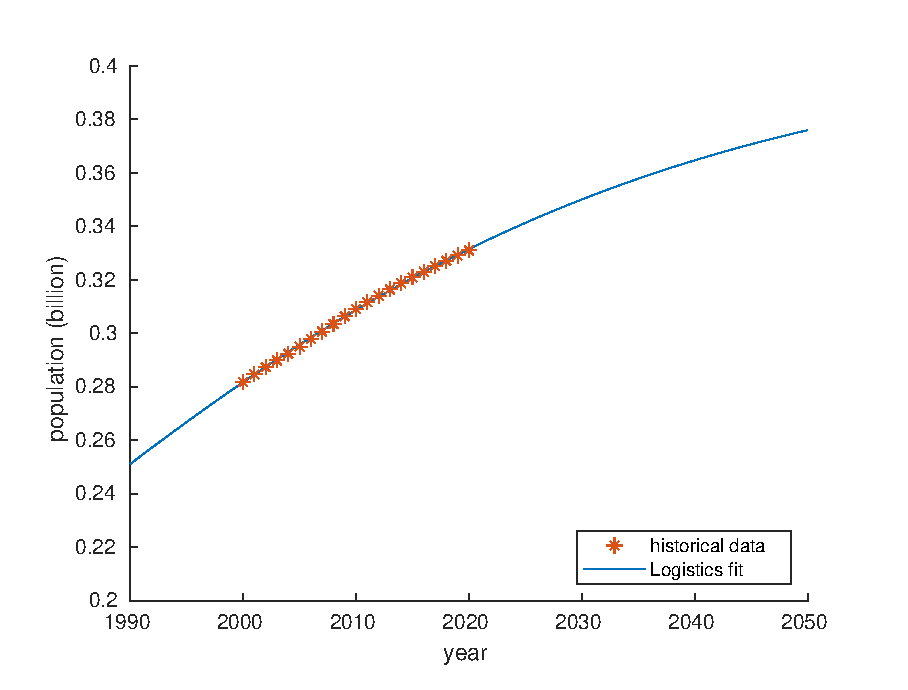
\includegraphics[width=0.9\textwidth]{figure/model/USA/USA_pplt.eps}
        \caption{Logistic Fit of Population of USA.\label{fig:USA_pplt}}
    \end{minipage}
    \begin{minipage}[t]{0.48\textwidth}
        \centering
        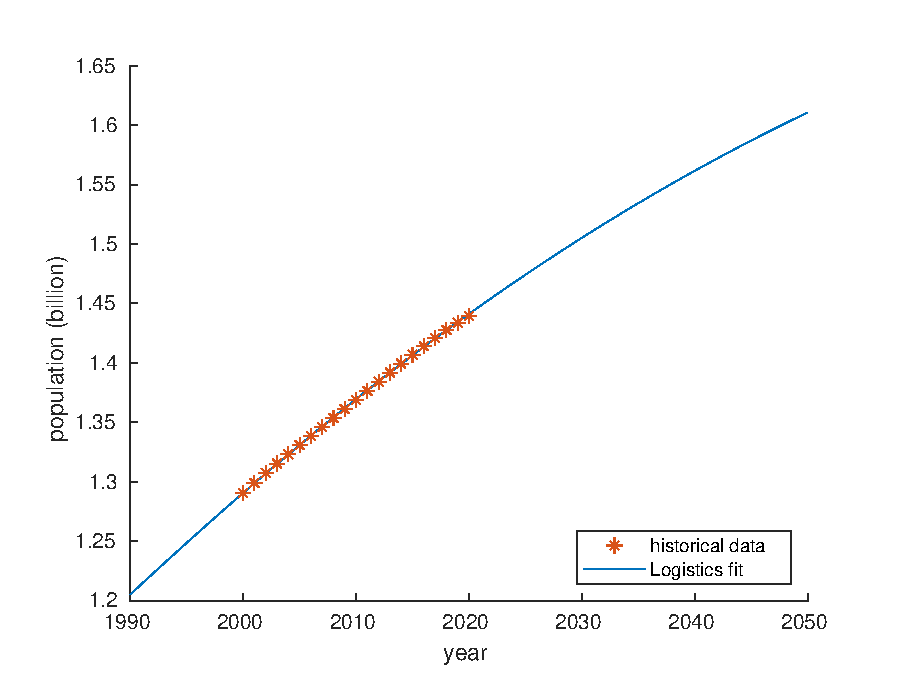
\includegraphics[width=0.9\textwidth]{figure/model/China/China_pplt.eps}
        \caption{Logistic Fit of Population of USA.\label{fig:China_pplt}}
    \end{minipage}
\end{figure}

%%%%%%%%%%%%%%%%%%%%%%%%%%%%%%
\subsection{Model for evaluating \textit{EF}} \label{sec:EF}

Stockholm Environment Institute defines the efficiency in the food system as ``the ratio of outputs to inputs'' \cite{cite:Efficiency_1}. However, to estimate factors of input and output of different kinds of food requires a huge set of data from measurements and experiments, and from all the literature we read no one even try to explore the overall efficiency of a complex food system. We finally select the sum of the annual food yield of different food as an indicator for efficiency. The selection of the indicator refers to work by \cite{cite:Esti_efficiency}. 

In order to calculate the value of efficiency in the food system we choose, we do the following steps:

\begin{itemize}
    \item \textbf{Find the total yield.} Based on the food pyramid provided by a Harvard research \cite{cite:Food_pyramid}, we divide food into six groups: cereal, fruit, oil crops, vegetable, dairy, and meat. The total food yield is given by Formula \eqref{eq:yield} below.
    
    \begin{align}
        \label{eq:yield} S = \sum^6_{i=1}s_i, \text{ where }s_i\text{ is the yield of the i-th food.}
    \end{align}
    
    \item \textbf{Determine the target yield in year $t$.} Consider the malnutrition rate and obesity rate among adults, the value of the target yield in the i-th year $S_m(t)$ can be obtained by Formula \eqref{eq:target} below.
    
    \begin{align}
        \label{eq:target} S_m(t) = \frac{S_{2020}/(1+OR_{2020}-UR_{2020})}{p_{2020}}\cdot p(t).
    \end{align}
    
    \item \textbf{Establish the equation for yield $S(t)$.} In the equation we introduce a coefficient $PM$, called policy motivation, to reflect the regulation of priorities. First, our aim is to ensure that the larger $PM$ is, the greater the efficiency $EF$ changes. Second, we anticipate that if the current food yield $S$ is larger than the target yield $S_m$, $S(t)$ will decrease with respect to time $t$, and if the current $S$ is less than the target yield $S_m$, $S(t)$ will increase with respect to time $t$. Third, the first two changes should be applied to food yield $S(t)$ itself. Then we obtain Equation \eqref{eq:logi}, which is similar to the equation of logistic model, but \textbf{the denominator in the middle entry is now a variable, instead of a constant}: 
    
    
    \begin{equation}
    \left\{
    \begin{aligned}
        \label{eq:logi} & \frac{\mathrm{d} S}{\mathrm{d} t} = PM\cdot  (1-\frac{S(t)}{S_m(t)})\cdot S(t) \\
        & S_{\text{initial}}  =  S_{2020} \\ 
    \end{aligned}
    \right.
    \end{equation}

    \item \textbf{Solve the differential equation.} In order to obtain the numerical solution of this differential equation, we adopt \textbf{Runge-Kutta method} for the initial-value problem \cite{cite:Runge}. First, we separate the interval $[2020, 2050]$ (indicating the year from 2020 to 2050 as our evaluation range) into $N$ sub-intervals $[t_n, t_{n+1}]$ ($n = 0, 1, \cdots, N-1$). Then, by the mean value theorem we have 
    
    \begin{align}
        S(t_{n+1}) - S(t_n) = \int^{t_{n+1}}_{t_n} f(t,S(t)) \mathrm{d}t = (t_{n+1}-t_{n}) f(\xi, S(\xi)), \text{where }\xi\in [t_n, t_{n+1}] \text{\cite{cite:Runge}}.
    \end{align}
    
    Finally, by approximation we get 
    
    \begin{align}
        S_{n+1} -S_n = (t_{n+1}-t_n) \sum^m_{i = 1} c_i f(\xi_i, y(\xi_i)), \text{where we choose }m = 4, c_1 = c_4 =1/6, 
    \end{align}
    
    and $c_2 = c_3 = 1/3$.
    
    \item \textbf{Normalize the result.} After obtaining results of the total yield, we rate the values by making a \textbf{min-max normalization}. The form is shown in Formula \eqref{eq:Normal}.
    
    \begin{align}
        \label{eq:Normal} EF(t) = \frac{S(t)-S_{\min}}{S_{\max}-S_{\min}}
    \end{align}
\end{itemize}

%%%%%%%%%%%%%%%%%%%%%%%%%%%%%%%%
\subsection{Model for evaluating \textit{EQ}}

According to the literature found on the database \cite{cite:Equity_def, cite:Equity_def2}, equity problems in the food system includes racism, gap between the rich and the poor, gender inequality, etc. In our model for the food system, since we take each country as a unit, we are aimed at regarding a country as a whole and finding the difference between countries. 

Therefore, for all studied objects, we assume that categories in the dietary structure are totally included by the types of agricultural products produced, which is actually mostly the case. Therefore we claim that countries we selected can be \textbf{self-sufficient} in food categories. We then come up with a method making full use of the outcomes of Subsection \ref{sec:EF}. 

We use \textbf{the ratio of supply and demand $S(t)/S_m(t)$} to denote the level of equity. The interpretation comes from the fact that if the current total yield is close to the target yield then everyone in the country has a chance to have the necessary amount of food, neither too excessive (which implies that there are some people in the country possess the food amount more than they need) nor too insufficient (which implies that there are some people in the country possess the food amount less than they need). Finally, we normalize the result in the same procedure as what is shown in Subsection \ref{sec:EF}.


%%%%%%%%%%%%%%%%%%%%%%%%%%
\subsection{Model for evaluating \textit{PF}} \label{sec:pf}

The profitability in the food system can be defined as the \textbf{total income} by selling all the food in terms of their different prices. Besides, the price by prediction should have limits in the scope of value to prevent price mutations in a certain year. We assume that people are rational enough to always pursue the maximum profit. Therefore, we use \textbf{linear programming} to solve this problem. 

Formula \eqref{eq:profit} shows the calculation form. For the constraints on linear programming problems, we stipulate the yields of each food \textbf{within the yields interval for recent five years}, so that we can ensure the continuity of the yields. For the future price of food, we apply \textbf{linear fit} to each kind of food to predict.


\begin{gather}
% 
% \centering
\max \quad  \sum_{i=1}^{6} (s_i \frac{PR_i}{IF}), \notag\\
\mbox{s.t.} \quad 
\sum_{i=1}^{6} s_i =S(t),\label{eq:profit} \\
\min \{ \frac{s_k(t-j)}{S(t-j)} \} \leq \frac{s_k(t)}{S(t)} \leq \max \{ \frac{s_k(t-j)}{S(t-j)} \}, j=1,2,3,\ldots,5, \quad k = 1,2,3,\ldots,6. \notag
\end{gather}
% &\min \{ \frac{s_2(t-j)}{S(t-j)} \} \leq \frac{s_2(t)}{S(t)} \leq \max \{ \frac{s_2(t-j)}{S(t-j)} \},&j=1,2,3\ldots,5 \\
% &\min \{ \frac{s_3(t-j)}{S(t-j)} \} \leq \frac{s_3(t)}{S(t)} \leq \max \{ \frac{s_3(t-j)}{S(t-j)} \},&j=1,2,3\ldots,5 \\
% &\min \{ \frac{s_4(t-j)}{S(t-j)} \} \leq \frac{s_4(t)}{S(t)} \leq \max \{ \frac{s_4(t-j)}{S(t-j)} \},&j=1,2,3\ldots,5 \\
% &\min \{ \frac{s_5(t-j)}{S(t-j)} \} \leq \frac{s_5(t)}{S(t)} \leq \max \{ \frac{s_5(t-j)}{S(t-j)} \},&j=1,2,3\ldots,5 \\
% &\min \{ \frac{s_6(t-j)}{S(t-j)} \} \leq \frac{s_6(t)}{S(t)} \leq \max \{ \frac{s_6(t-j)}{S(t-j)} \},&j=1,2,3\ldots,5 \\


Finally, we normalize the result in the same procedure as what is shown in Subsection \ref{sec:EF}.


\subsection{Model for evaluating \textit{SU}}

According to Holden et al. \cite{cite:Sus1}, the excessive consumption of fossil fuel is one of the most severe influence current food systems have on the natural environment, and causing the food system unsustainable. Hence, we choose the total emissions from agriculture in one country as an indicator of the sustainability. Considering the fact that the larger food production is, the more emissions from agriculture will be, we take the quotient, i.e., the emissions per unit of the yield, to reflect the performance of sustainability. We should also take the policy motivation into account:

\begin{itemize}
    \item Before the policy change, we do \textbf{liner fittings} for the data of greenhouse gas emissions and the data of total yield per year we collected respectively. Figure \ref{fig:lf_E_yield_GHG} shows the fitting performance of greenhouse gas emission and annual yield. The coefficients of determination of linear fit of them are $0.9706$ and $0.9603$ respectively, which are very close to the ideal value $1$. Equations \eqref{eq:lf_E_GDG} and \eqref{eq:lf_E_yield} show the fitting results.
    \begin{figure}[htbp]
        \centering
    	\subfigure[Linear Fit of the Annual Yield of Ethiopia.]{\includegraphics[width=0.48\textwidth]{figure/model/Ethiopia/Ethiopia_yield_fit.eps}} 
    	\subfigure[Linear Fit of the Greenhouse Gas Emmision of Ethiopia.]{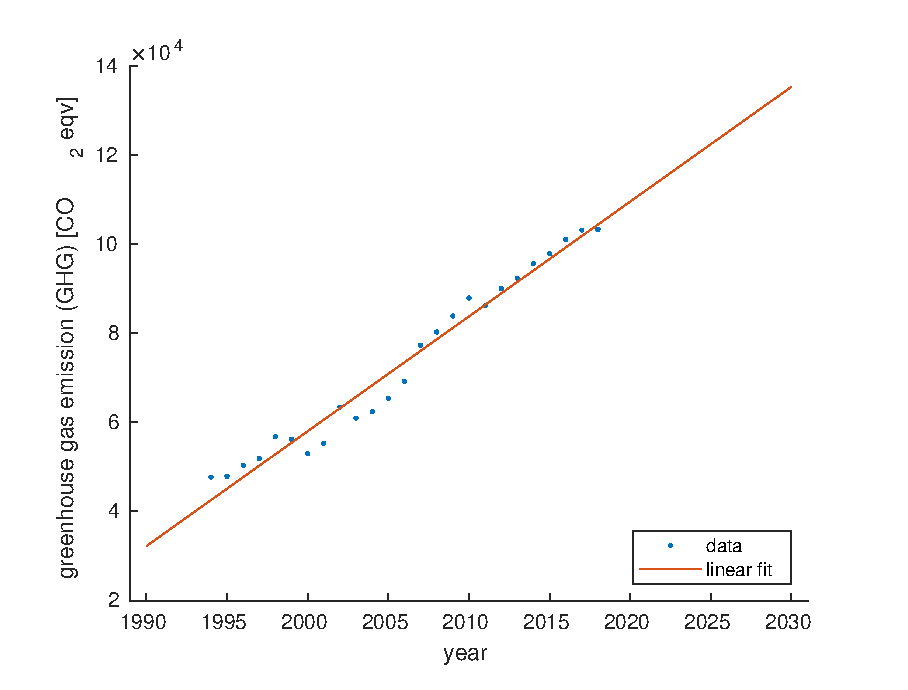
\includegraphics[width=0.48\textwidth]{figure/model/Ethiopia/Ethiopia_GHG_fit.eps}} 
        \caption{Sensitivity Test for Policy Motivation \textit{PM}.\label{fig:lf_E_yield_GHG}}
    	\vspace{0.2in}
    \end{figure}
    \begin{gather}
        GHG(t) = a\cdot t - b, \text{where } a = 2576, b = 5.049\times10^6 \label{eq:lf_E_GDG}\\
        S(t) = c\cdot t - d, \text{where } c = 1.228\times10^6, d = 2.443\times10^9 \label{eq:lf_E_yield}
    \end{gather}
    Then we have the expression below:
    
    $$\frac{GHG(t)}{S(t)} = \frac{a t-b}{c t-d}.$$
    \item \textbf{Modify the equation.} After the policy change, we take $PM$ into account, and update the expression as below (suppose the policy change occurs in 2020):
    
    $$\frac{GHG(t)}{S(t)} = \frac{a (t-2020) + (2020 a -b)(1-PM)}{c (t-2020) + (2020 c - b)(1-PM)},$$
    
    from where we should notice that the new function has \textbf{the same asymptotic line as the older one} (which is $y = a/c$ as $x\to \infty$), and the two functions \textbf{intersect at \textit{t = 2020}}. The new function also indicates that \textbf{when \textit{PM} = 0 the two functions are equal}, and given a stronger policy motivation $PM$ the new function will drop more steeply.
\end{itemize}

After we predict the value of sustainability by year, we normalize the result in the same procedure as what is shown in Subsection \ref{sec:EF}.

\subsection{Model for evaluating \textit{PFSI}}
We obtain the prioritized food system index $PFSI$ by making weighted summation of $EF$, $EQ$, $PR$, and $SU$. Values of weight are obtained through \textbf{Analytic Hierarchy Process (AHP)}. To reasonably indicate the main focus of the food system, we define Formula \eqref{eq:PFSI} below to find the value of $PFSI$:

\begin{align}
    \label{eq:PFSI} PFSI(t) = (1-EF(t))\cdot r_1 + (1-PR(t))\cdot r_3 + EQ(t)\cdot r_2 + SU(t)\cdot r_4
\end{align}

It is suggested that \textbf{when \textit{PFSI} is closer to 0 the focus of the food system is more on \textit{EF} and \textit{PR}}, and \textbf{when \textit{PFSI} is closer to 1 the focus of the food system is more on \textit{SU} and \textit{EQ}}.

%图?

The steps of calculating weights by \textbf{AHP} are shown below:
\begin{itemize}
    \item We first determine the relative significance of four factors (\textit{EF}, \textit{PF}, \textit{EQ}, and \textit{SU}). Specifically, \textit{EF} and \textit{PF} are considered to have the same significance, and \textit{EQ} and \textit{SU} are considered to have the same significance. We set the the significance of \textit{EQ} (or \textit{SU}) with respect to \textit{EF} (or \textit{PF}) to be $rs$. Then, the comparison matrix $A$ (Equ. \eqref{eq:comM}) is set up.
    \begin{equation}
        A=\left[\begin{array}{cccc}
        1 & 1 & 1/rs & 1/rs \\
        1 & 1 & 1/rs & 1/rs \\
        rs & rs & 1 & 1     \\
        rs & rs & 1 & 1
        \end{array}\right]
        \label{eq:comM}
    \end{equation}
    In the case study (Sec. \ref{sec:case}), we set $rs = 7$. However, the absolute value of $rs$ does not affect the general shape of the final result, which will be verified in sensitivity analysis (Sec. \ref{sec:sense}).
    \item Calculated the eigenvalues of matrix $A$, we can further determine the weights of \textit{EF}, \textit{PF}, \textit{EQ}, and \textit{SU} by normalize the eigenvector of the maximum eigenvalue. Namely, the weight vector can be calculated through Equ. \eqref{eq:AHPweight}.
    \begin{equation}
        \mathbf{w} = \frac{\mathbf{v}}{\|\mathbf{v}\|_1} = \frac{\mathbf{v}}{\sum_{i=1}^4|v_i|}
        \label{eq:AHPweight}
    \end{equation}
    \item To prevent the possible conflict caused by arbitrarily set significance, we are supposed to assess the validity of the weights. We define the consistency index $CI$ as
    \begin{equation}
        CI = \frac{\lambda - 4}{4-1} = \frac{\lambda - 4}{3},
    \end{equation}
    where $\lambda$ is the maximum eigenvalue of comparison matrix $A$. Then, the consistency ratio $CR$ can be calculated through
    \begin{equation}
        CR = \frac{CI}{RI},
    \end{equation}
    where $RI$ is random consistency index. Here, we have 4 factors in total, so $RI=0.9$. In general, if $CR<0.1$, the weights obtained from AHP is valid.
\end{itemize}

\section{Discussion}
\subsection{Task 1: Re-Optimization for the Food System}

Since there are interactions among the model for efficiency, profitability, sustainability, and equity, after the optimization for equity and sustainability we need to look at the consequence of the changes of their weight. We consider the situation in different countries. 

\begin{itemize}
    \item \textbf{For a country in which the undernourishment rate is less than the obesity rate, we claim that the total food production amount is enough to satisfy the need of all the population.} The country produces food surpluses. As a result, under the influence of policy motivation, the country will tend to produce exactly the amount of food they need, so that the total yield of food \textbf{will decrease at first}, causing a decline of $EF$. When the intermediate rate state is reached, the prediction of the level of efficiency will depend on the population change as well. In the countries where the population is growing continuously, the annual food yield should try to catch up with the population, and accordingly \textbf{the total yield and $EF$ will increase since then}. In the countries where the population is declining, the change will be in the opposite case.
    
    Besides, the value of the level of \textbf{equity ($S/S_m$) will decrease to 1} at first since the food yield is large. According to the differential equation, we can see that at this time the growth rate of the yield is 0. Hence, the value of $S/S_m$ will go on decreasing until less than 1. However, the slope of $S$ will be higher until it surpasses the population growth rate, so that \textbf{in the end $S/S_m$ will approach to 1}, implying that the amount of food per person is more equitable. 
    
    As for the profitability, since the prices of each kind of food is not fixed, these prices are predicted by linear fitting. However, one thing is known that we use the yields interval for recent five years for the linear programming, so that we may infer from the expression that \textbf{the level of profitability will change smoothly}. Another supporting argument is that we aim to find the maximum income for each year so that the \textbf{food system still seek for the maximum benefits even sustainability is considered now}.
    
    For the prediction of the change of sustainability, we can find that the \textbf{greenhouse gas emissions keep increasing in developing countries} like China, and remain nearly constant in developed countries like the USA. Then after exerting policy motivation, \textbf{the value of $GHG(t)/S(t)$ will decrease faster than the case before re-optimization}. However, for our model in the end the level of sustainability will be the same as before because the two functions have the same asymptotic line. It reflects that this model loses some accuracy for a very long term prediction.
    
    
    \item \textbf{For a country in which the undernourishment rate is higher than the obesity rate}, the total food production amount is not enough. In this case, the total yield will be raised to meet the need for food by residents. If the population growth rate is larger than \textbf{$PM$, $S/S_m$ will be firstly less than 1 then approach 1}. In the end, the population reaches its limit, and correspondingly the yield will approach approximately a constant.
    
    On the contrary, \textbf{if the population growth rate is less than $PM$}, then $S/S_m$ will decline due to the fact that the yield does not catch up with the rate of population growth. When the population growth rate begins decreasing, $S/S_m$ will rise up again until leveling off to 1.
    
    The analysis of profitability and sustainability is the same as above.
    
\end{itemize}


\textbf{We define 0.5 as the balance value for efficiency, profitability, equity, and sustainability.} It means that we regard them as equally important. According to our model, the time that a food system needs to implement should be counted from the occurrence of policy change to the moment when $PFSI$ reaches 0.5 from either side for the first time. The interpretation is that when $PFSI > 0.5$ indicators including sustainability and equity become more important than efficiency and profitability. 

%%%%%%%%%%%%%%%%%%%%%
\subsection{Task 2: Benefits and Costs}

We only consider the case of changing the priorities of a food system from efficiency and profitability to sustainability and equity. The opposite direction will give the contrary result. 

\subsubsection{Potential benefits}

\begin{itemize}
    \item \textbf{Distribution become more reasonable within developed countries, and will first receive a drop in some developing countries, but later will recover.} When we change the prioritization of food system to sustainability and equity, it is obvious that \textbf{ developed countries will tend to distribute its food more fairly} among its residents, because the equity is always approaching 1. However, for some developing countries, Ethiopia, for example, firstly received a drop in equity. This can result from the fact that the production rate fails to exceed the population rate at first. But later, equity of developing countries will approach 1 again as the production rate increases and the population growth rate decreases.
    \item \textbf{Under the motivation of policy, sustainability for both developed countries and developing countries become stronger.} As it will also \textbf{limits the increase of emission amount of greenhouse gas} if the total yields grow. Such effect becomes \tetxbf{mostly apparent in the developed country}, as the obesity rate is much larger than the undernourishment rate, and the yield generally decreases. While in some developing country, which has a large undernourishment rate, yield growth is also limited with stronger sustainability, so that the atmosphere and environment are protected, and used more efficiently.
\end{itemize}

\subsubsection{Potential costs}
\begin{itemize}
    \item \textbf{Developing countries will become tougher when cooperating with the increase of the population} For some developing countries, whose obesity rate is slightly larger than the undernourishment rate, they will first drop the yields to fit the current population and then try to keep pace with the population growth. Comparing with such a "following" strategy, if countries try to increase their yields at first to cope with the future population, they will become more prepared.
    
    \item \textbf{Profit from the food industry will always decrease regardless of developed and developing countries.} In the later case study section, we illustrate the change of profitability, and these charts show that all developed and developing countries received profit loss. On one hand, this can result from some yield drop in some developed countries. On the other hand, some developing countries have a relatively large inflation rate, causing the actual profit to become less valuable. 
\end{itemize}

\subsubsection{Prediction on the occurrence of the benefits and costs}
Here, we firstly define \textbf{the occurrence of the previously mentioned benefits and costs as the time when equity is within the interval [0.95,1.05] and is continuously monotonically increasing/ monotonically decreasing to approach 1}. With that definition and referring to the findings in section \ref{sec:case}, we can find that China's occurrence time happened in the approximately year 2045 and that Ethiopia's occurrence time happened in the approximately year 2025, while America's occurrence time happened in the approximately year 2051. Therefore, with these experiment result, we can qualitatively conclude that \textbf{the occurrence time of developed countries is later than the developing countries under the same policy motivation (PM)}.

%%%%%%%%%%%%%%%%%%%%%
\subsection{Task 3: Case Studies}\label{sec:case}

Instead, we need to utilize the prediction result of food prices and greenhouse gas emissions. Here we only show the plot of the scores for each indicator by using the method mentioned before. 

\subsubsection{China: Developing Country with $UR_{2020}$ relatively less than $OR_{2020}$}
China is the representative developing country whose economic situation is very close to some developed countries. Specifically, the undernourishment rate of China is much smaller than the obesity rate in year 2020. This fact reflected a high possibility that the food China produced is more than the demand of people. However, as a developing country, its population is still in the quickly rising period. Thus, \textbf{the current supply of food can not satisfy the demand of its future maximum population}. To satisfy the food demand of current population, \textbf{the yield amount will firstly receive a slight drop until year 2035. But after that, the yield will continuously increase to follow the increase of population and corresponding demand.} Figure \ref{fig:China_yield} shows the predicted situation with policy motivation. This result is obtained from the model for evaluating \textit{EF} with \textit{PM}$=0.1$. Meanwhile, the equity of food will be improved due to a better arrangement of supply. As the annual yield is controlled by the policy, the supply is gradually close to the demand (Fig. \ref{fig:China_equity}), which ensures the domestic equity of food system. As shown in the Figure \ref{fig:China_yield} and \ref{fig:China_equity}, the effect of the policy will reach the maximum at approximately year \textbf{2035}, namely, 15 years after the implementation of policy. After about \textbf{25 years} of continuously policy motivation, the re-optimized food system is finally set up. \textbf{At that time, the ratio of supply demand is extremely close to 1 and the yield is almost constant.}
\begin{figure}[htbp]
    \centering
    \begin{minipage}[t]{0.48\textwidth}
        \centering
        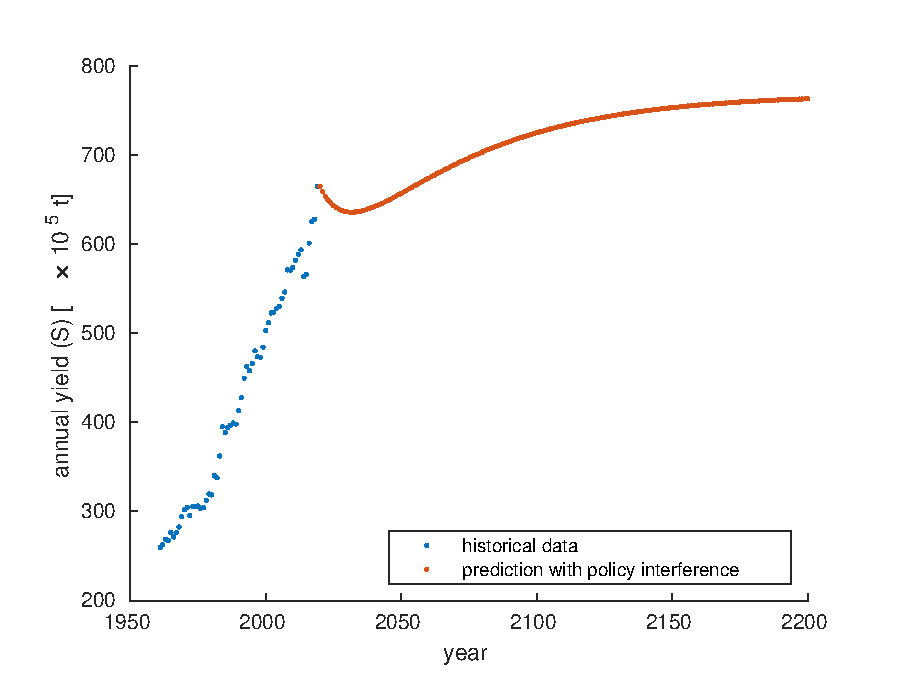
\includegraphics[width=0.9\textwidth]{figure/model/China/China_yield.eps}
        \caption{Annual Yield of China with Policy Interference.\label{fig:China_yield}}
    \end{minipage}
    \begin{minipage}[t]{0.48\textwidth}
        \centering
        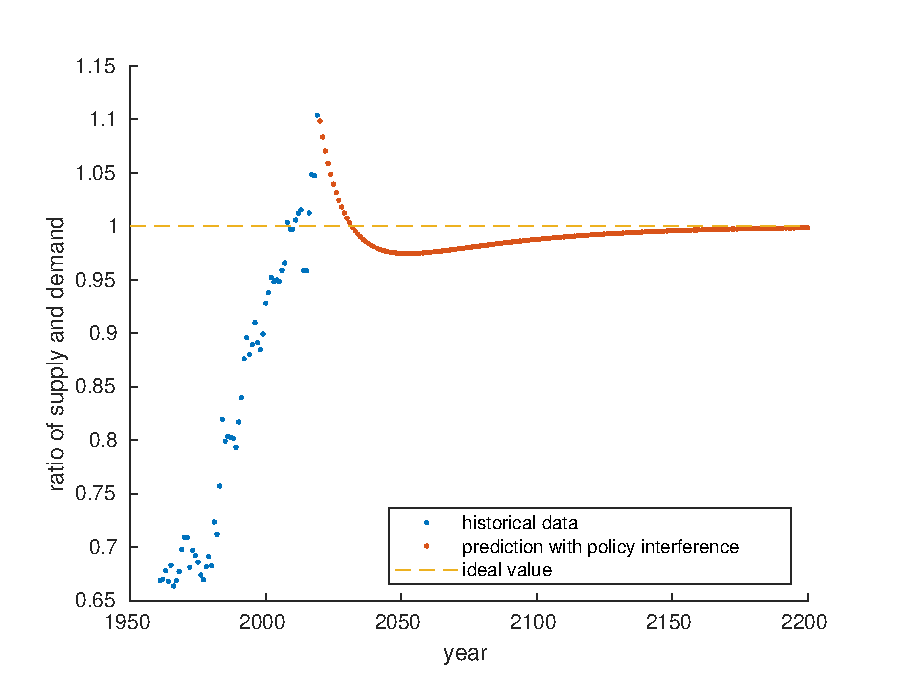
\includegraphics[width=0.9\textwidth]{figure/model/China/China_equity.eps}
        \caption{Ratio of Supply and Demand of Food of China with Policy Interference.\label{fig:China_equity}}
    \end{minipage}
\end{figure}

Besides, the policy will have a \textbf{negative effect on the income} of the people served in the food system and a \textbf{positive effect on the sustainability} of the food system. Due to the effect of inflation, the short-term decrease of yield will result in a \textbf{continuous attenuation of the income}. Using the model stated in Section \ref{sec:pf}, we can predict the income (Fig. \ref{fig:China_income}). Furthermore, the policy will also \textbf{push the development of science} in order to decrease the labor cost. This in turn improves the production method such that less greenhouse gas emission is necessary for the same yield. Red line in figure \ref{fig:China_GHG} shows the \textbf{accelerated decreasing trend greenhouse gas emission} with policy motivation. 
\begin{figure}[H]
    \centering
    \begin{minipage}[t]{0.48\textwidth}
        \centering
        \includegraphics[width=0.9\textwidth]{figure/model/China/China_profit.eps}
        \caption{Income of Food System of China with Policy Interference.\label{fig:China_income}}
    \end{minipage}
    \begin{minipage}[t]{0.48\textwidth}
        \centering
        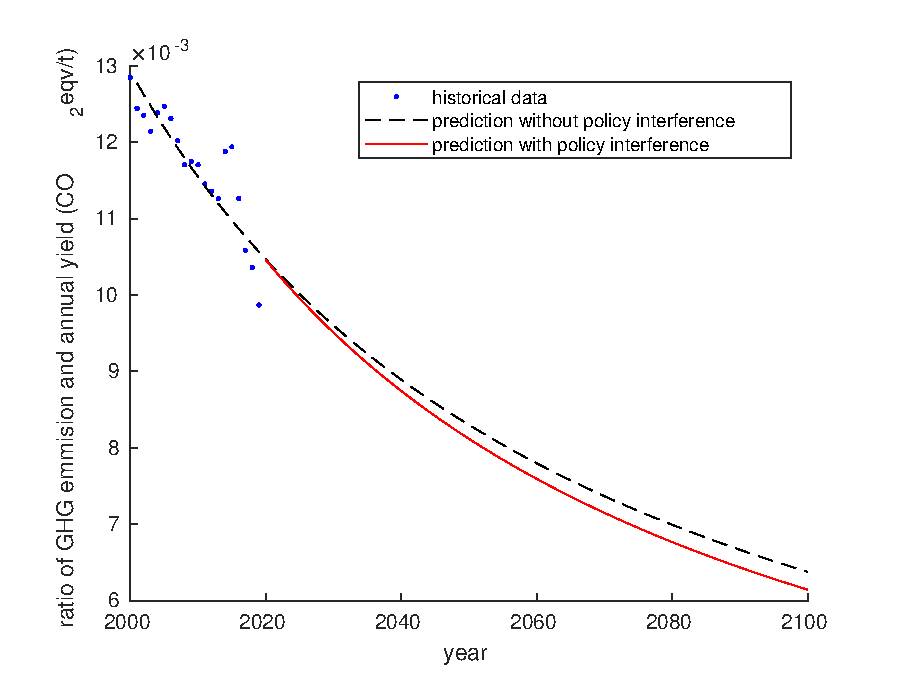
\includegraphics[width=0.9\textwidth]{figure/model/China/China_sustainability.eps}
        \caption{Greenhouse Gas Emission per yield of the Food System of China with Policy Interference.\label{fig:China_GHG}}
    \end{minipage}
\end{figure}

Finally, with the economic, social, scientific, and environmental factors taken into account, the food system in China will prioritize equity and sustainability \textbf{after the 15 years} of implementation of the policy. With \textbf{10 more years} of development, the benefits and the costs of the new food system will be manifest. Figure \ref{fig:China_score} shows the change of evaluated \textit{PFSI} with \textit{EF}, \textit{PF}, \textit{EQ}, and \textit{SU} marked. Figure \ref{fig:China_radar} shows the standardized score of \textit{EF}, \textit{PF}, \textit{EQ}, and \textit{SU} in 2021, 2035 (15 years after policy's implementation), 2045 (25 years after policy's implementation).
\begin{figure}[!htb]
    \centering
    \begin{minipage}[t]{0.48\textwidth}
        \centering
        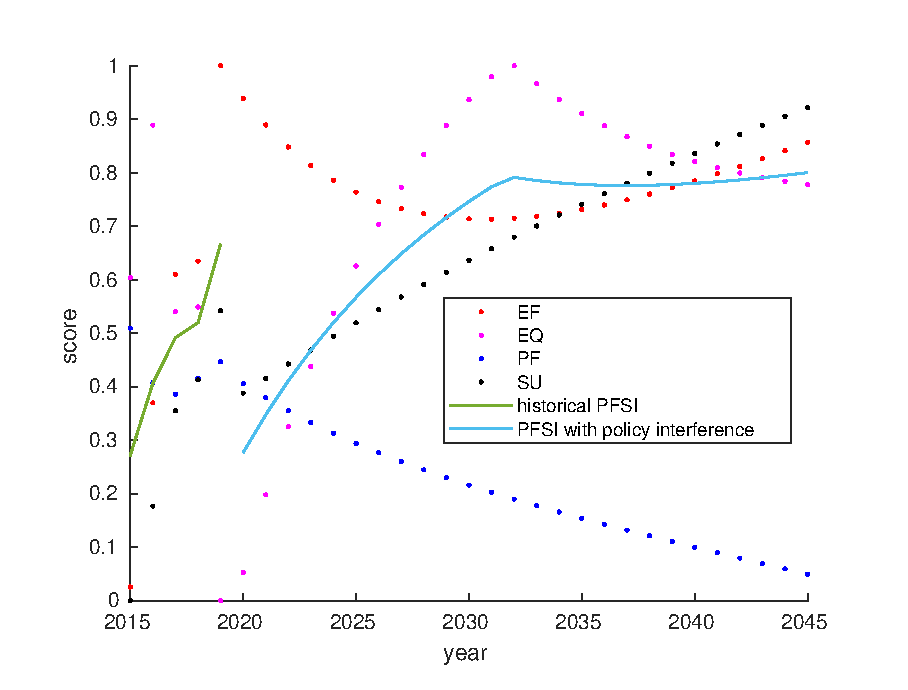
\includegraphics[width = 0.8\textwidth]{figure/model/China/China_score.eps}
        \caption{\textit{PFSI} of China with All Four Factors Specified from 2015 to 2045.\label{fig:China_score}}
    \end{minipage}
    \begin{minipage}[t]{0.48\textwidth}
        \centering
        \includegraphics[width = 0.8\textwidth]{figure/radar/China_radar.pdf}
        \caption{The Change of Four Factors of China's Food System.\label{fig:China_radar}}
    \end{minipage}
\end{figure}

\subsubsection{Ethiopia: Developing Country with $UR_{2020}$ larger than $OR_{2020}$} 
Ethiopia is a typical developing country with a high undernourishment rate and low obesity rate. Therefore, the current food supply of Ethiopia is far away from the demand of its possible maximum population. As we change the priority of the food system by introducing the policy motivation, the annual yield will \textbf{quickly increase to satisfy the demand of the population} (Fig. \ref{fig:Ethiopia_yield}). As for the equity, policy motivation \textbf{inhibits increasing speed of equity} to prevent it exceeds the ideal value $1$. Similar to Ethiopia, the income will be affected by the policy so that it \textbf{decreases quickly at the beginning of the policy's implementation}. However, due to the large inflation rate, the \textbf{decreasing speed is much larger} than in China. Besides, the sustainability of Ethiopia will also be improved with the policy motivation. The biggest difference between China and Ethiopia is the value of policy motivation \textit{PM}. To obtain the same effect as the food system of China, Ethiopia needs to \textbf{implement a much stronger policy regulation}. Through our estimation, the value of policy motivation of Ethiopia should be approximately 10 times that of China to get the same effect. In this case study, we choose to use policy motivation \textit{PM}$=1$.
\begin{figure}[htbp]
    \centering
    \begin{minipage}[t]{0.48\textwidth}
        \centering
        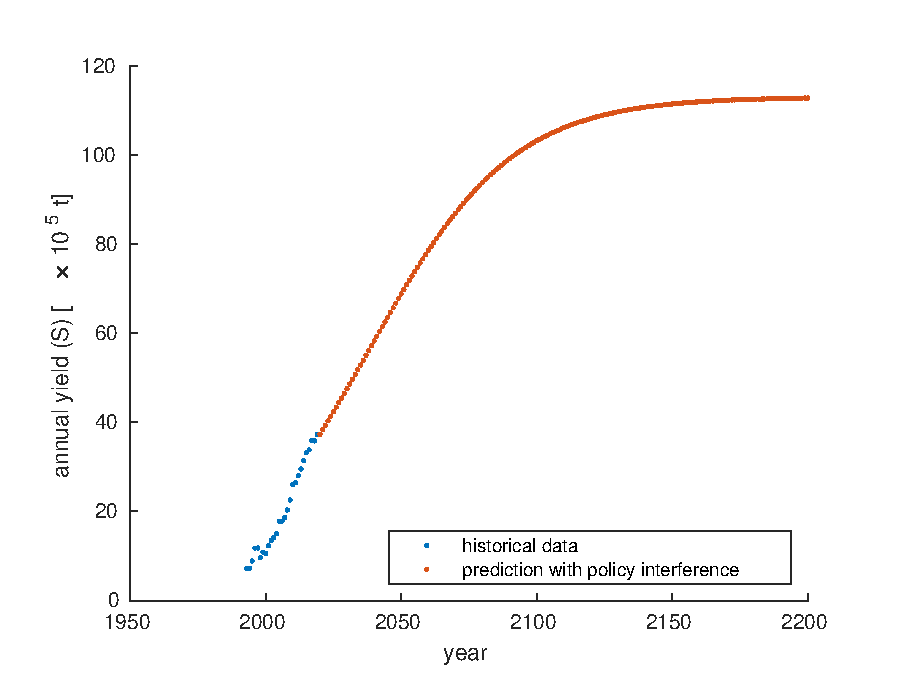
\includegraphics[width=0.9\textwidth]{figure/model/Ethiopia/Ethiopia_yield.eps}
        \caption{Annual Yield of Ethiopia with Policy Interference.\label{fig:Ethiopia_yield}}
    \end{minipage}
    \begin{minipage}[t]{0.48\textwidth}
        \centering
        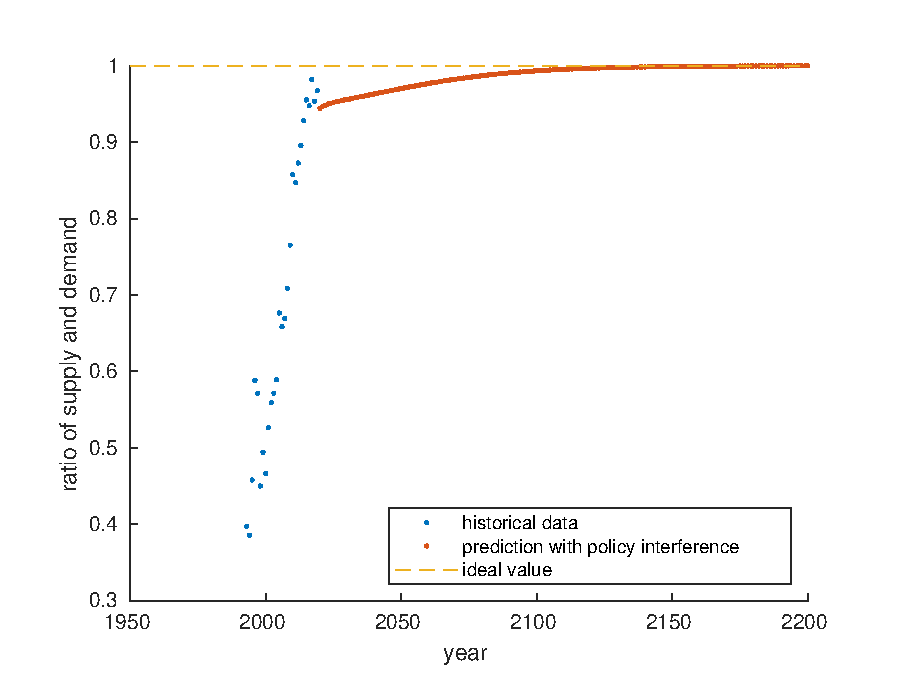
\includegraphics[width=0.9\textwidth]{figure/model/Ethiopia/Ethiopia_equity.eps}
        \caption{Ratio of Supply and Demand of Food of Ethiopia with Policy Interference.\label{fig:Ethiopia_equity}}
    \end{minipage}
\end{figure}

Finally, we calculate the line of \textit{PFSI}. After changing the weight of efficiency, profitability, equity, and sustainability, a gap appears in the year 2020. Different from China, the growth rate of Ethiopia's \textit{PFSI} is not that big. Instead, \textit{PFSI} \textbf{increases gradually in the beginning} and \textbf{is stable in year 2030}. Namely, only \textbf{10 years of policy motivation} can bring the underdeveloped food system of Ethiopia back to the right track, the balanced mode. Figure \ref{fig:Ethiopia_radar} shows the standardized score of \textit{EF}, \textit{PF}, \textit{EQ}, and \textit{SU} in 2021, 2035, and 2045.
\begin{figure}[!htb]
    \centering
    \begin{minipage}[t]{0.48\textwidth}
        \centering
        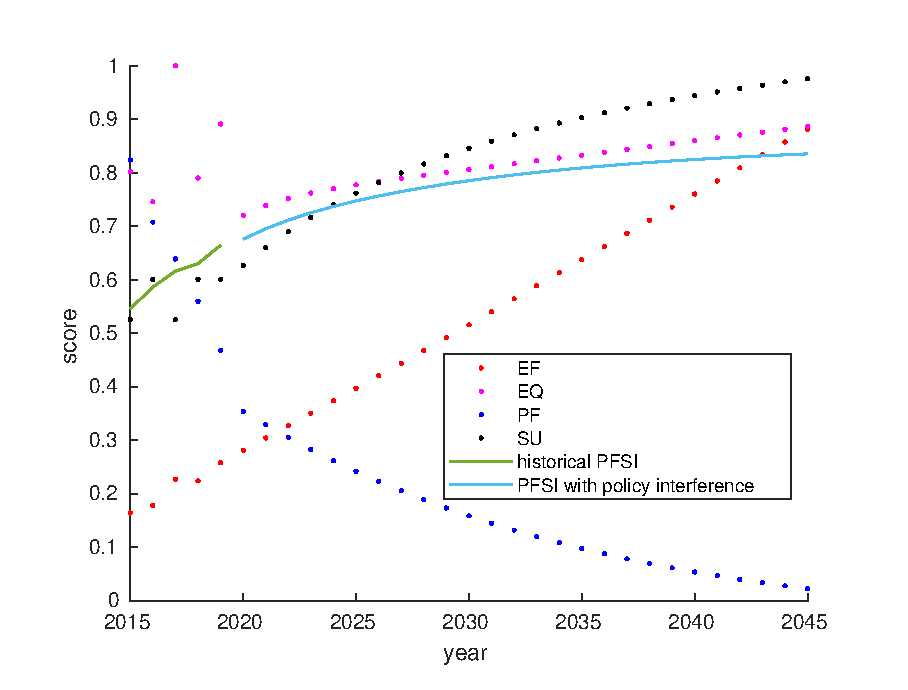
\includegraphics[width = 0.8\textwidth]{figure/model/Ethiopia/Ethiopia_score.eps}
        \caption{\textit{PFSI} of Ethiopia with All Four Factors Specified from 2015 to 2045.\label{fig:Ethiopia_score}}
    \end{minipage}
    \begin{minipage}[t]{0.48\textwidth}
        \centering
        \includegraphics[width = 0.8\textwidth]{figure/radar/Ethiopia_radar.pdf}
        \caption{The Change of Four Factors of Ethiopia's Food System.\label{fig:Ethiopia_radar}}
    \end{minipage}
\end{figure}

\subsubsection{The USA: Developed Country with $UR_{2020}$ much less than $OR_{2020}$}
The USA is a developed country where the undernourishment rate is very small while the obesity rate is very large. \textbf{Therefore, the current food supply of the USA even exceeds the demand of its possible maximum population.} After we change the priority to sustainability and equity, \textbf{the total yield amount (Fig. \ref{fig:USA_yield}) will generally receive a drop to satisfy the demand of population}, even in the year 2050, there will be a historically lowest point for the yields.  Moreover, as the equity index($S/S_m$) (Fig. \ref{fig:USA_equity}) is high at the present yield speed (about 1.4 in 2020), under the control of $PM$(policy motivation, set as 0.1), the equity will drop to 0.98 at the lowest level in the approximately year 2050 and then recover to 1 gradually so that it can compensate the increasing food demand caused by population growth. We can conclude that dropping the unnecessary yield of food can improve the sustainability of the food system, and increase equity in the long run.
\begin{figure}[htbp]
    \centering
    \begin{minipage}[t]{0.48\textwidth}
        \centering
        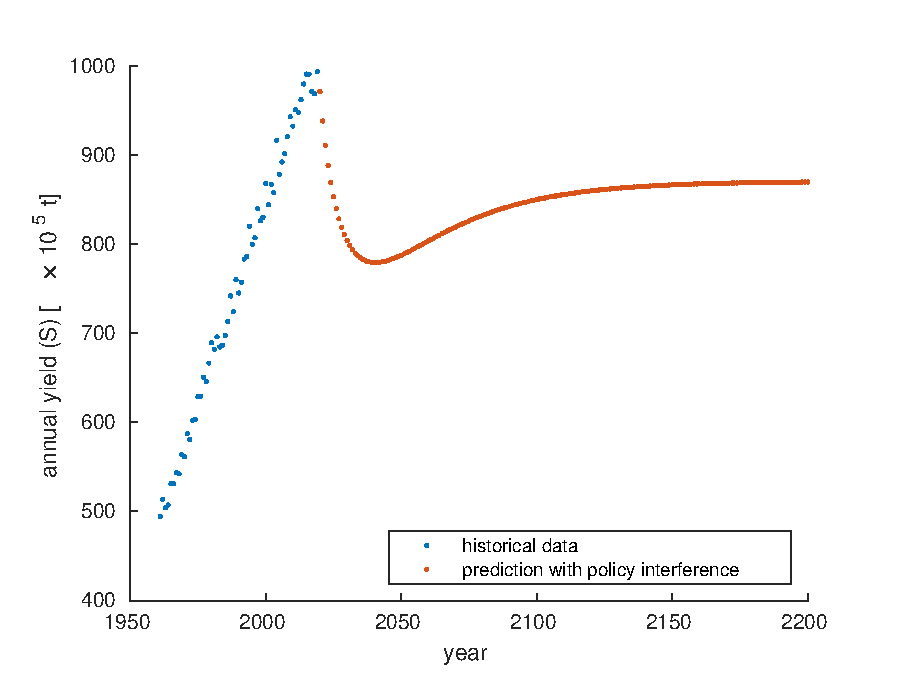
\includegraphics[width=0.9\textwidth]{figure/model/USA/USA_yield.eps}
        \caption{Annual Yield of USA with Policy Interference.\label{fig:USA_yield}}
    \end{minipage}
    \begin{minipage}[t]{0.48\textwidth}
        \centering
        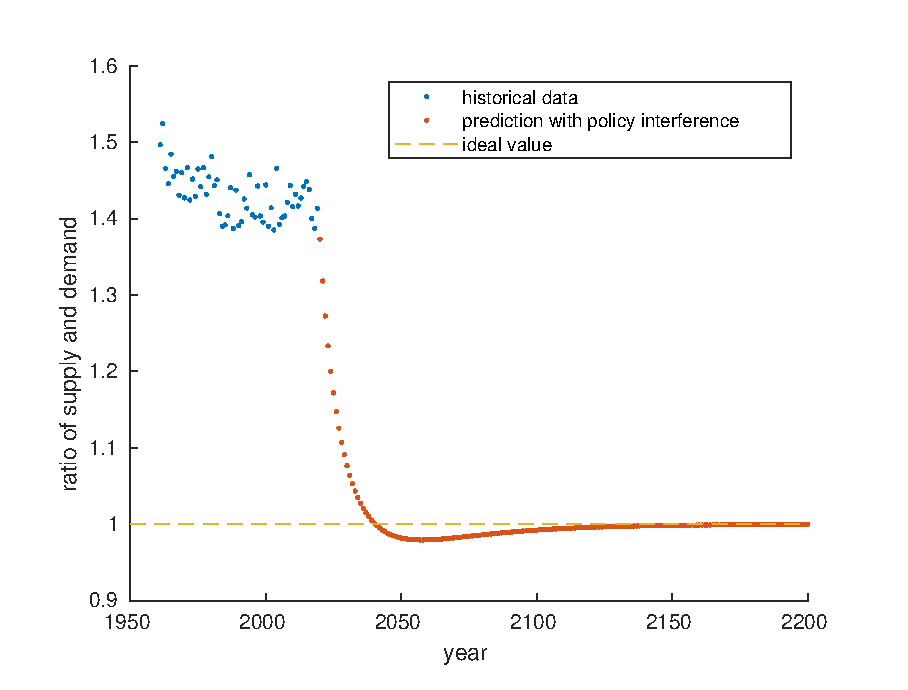
\includegraphics[width=0.9\textwidth]{figure/model/USA/USA_equity.eps}
        \caption{Ratio of Supply and Demand of Food of USA with Policy Interference.\label{fig:USA_equity}}
    \end{minipage}
\end{figure}

Similar to China, policy motivation will have a \textbf{negative effect on the income} of the people served in the food system due to the effect of inflation and price change. This is reasonable after taking the decrease in food yield into consideration. Besides, the ratio $GHG(t)/S(t)$ is also continuously drop with time. With the motivation of policy ($PM$=0.1), \textbf{the drops will be more quickly} comparing with the slope of $PM=0$.

Finally, we can calculate the line of $PFSI$ (figure\ref{fig:USA_score}). After changing the weight of equity, sustainability, profitability, and efficiency, a sudden drop happens in the year 2020. Then, \textbf{$PFSI$ will continuously grow} with its slope continuously drop. In approximately \textbf{the year 2027}, the scoring of $PFSI$ will exceed 0.5, which is the time the food system is optimized for equity and sustainability. In approximately \textbf{the year 2040},
efficiency received its historical highest point, and the differential of $PFSI$ received a sudden drop, which is the time the benefits and cost become manifest. Figure\ref{fig:USA_score} shows the standardized score of $EF$, $PF$, $EQ$, and $SU$ in 2021,2035, and 2045.


\begin{figure}[!htb]
    \centering
    \begin{minipage}[t]{0.48\textwidth}
        \centering
        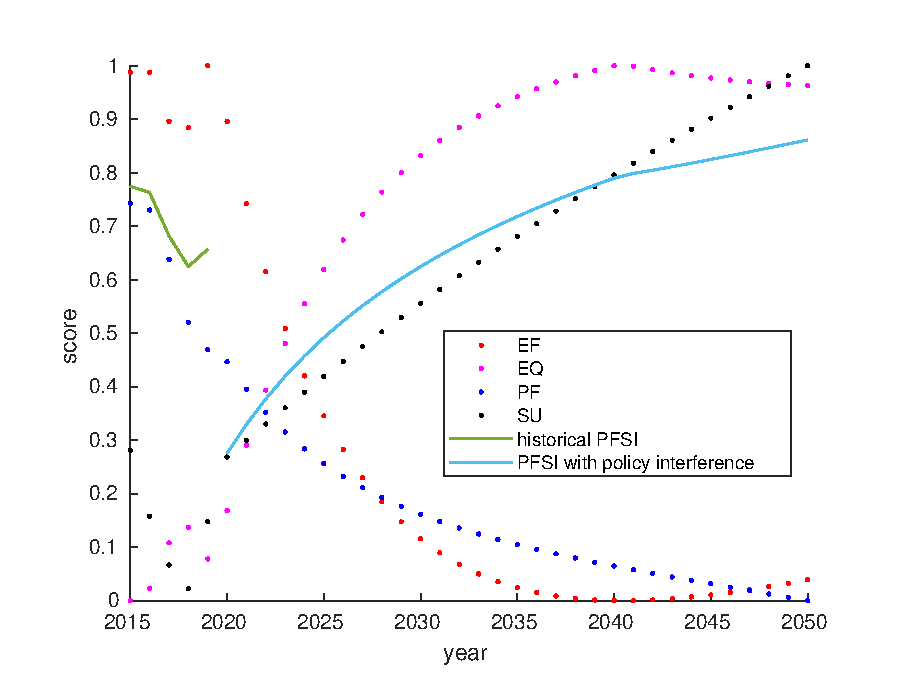
\includegraphics[width = 0.8\textwidth]{figure/model/USA/USA_score.eps}
        \caption{\textit{PFSI} of USA with All Four Factors Specified from 2015 to 2045.\label{fig:USA_score}}
    \end{minipage}
    \begin{minipage}[t]{0.48\textwidth}
        \centering
        \includegraphics[width = 0.8\textwidth]{figure/radar/USA_radar.pdf}
        \caption{The Change of Four Factors of USA's Food System.\label{fig:USA_radar}}
    \end{minipage}
\end{figure}







%%%%%%%%%%%%%%%%%%%%%
\subsection{Task 4: Scalability and Adaptability of the Model}

\subsubsection{Scalability}

Food systems with different scales are under consideration. After analysis, we make the following conclusions.

\begin{itemize}
    \item \textbf{The larger the food system is, the better our optimization will be}. Given a larger food system (major economies or unions of nations), the production structure of the food system will fit better with the common dietary structure for the residents. The reason is that we do not consider the food trade as well as other food communications between countries, and a larger scale can provide a more self-sufficient system.
    \item \textbf{Food systems of countries suit best}. Since the model is designed for countries, we consider the yearly inflation rate of a country in the model of profitability. The data processing may be revised if given other systems than countries.
\end{itemize}

\subsubsection{Adaptability}

Food systems with different properties are under consideration. Adaptability reflects the consequence when we change the object of the food system model. We have the following results.

\begin{itemize}
    \item \textbf{The model fits with countries with different $PM$}. For big countries like China and the USA, there is a large population along with strong scientific and technological support. However, for countries which have a smaller population and weaker policy support, the intensity of policy motivation needs to be modified to reflect the difference.
    \item \textbf{The model reflects the global polarization between rich countries and poor countries}. In Section \ref{sec:EF}, we include the undernourishment rate and the obesity rate into our evaluation model. With regard to Formula \eqref{eq:logi}, if $S_{2020}$ of a country is less than $S_m$, namely the average undernourishment rate is larger than the average obesity rate, then $1-S/S_m$ will be larger than 0. It indicates that the formula adapts to countries with different conditions of rich and poor.
    \item \textbf{The model is suitable for the comparison among countries with similar production capacity for food}. Since the costs in the production of food are neglected, the closer the production capacity among countries, the more comparable the result of profitability will be.
\end{itemize}


\section{Sensitivity Analysis}\label{sec:sense}
In our model, there are two variables whose value is set by us without derivation. They are the policy motivation \textit{PM} and the relative significance $rs$. \textit{PM} is set to $0.1$ in the cases of China and the USA and is set to $0.5$ in the cases of Ethiopia. $rs$ is set to $7$ in calculating weights of \textit{EF}, \textit{PF}, \textit{EQ}, and \textit{SU}. In this part, we will argue that the results we get from the model are not sensitive to the change of the values of \textit{PM} and $rs$.

\subsection{\textit{PM} Fluctuation Test.}
Policy motivation $PM$ represents the strength of policy in encouraging the balanced development of the food system. It is first used to calculate the annual yield and equity index in our model for a prioritized food system. We re-calculate the annual yield and equity index with a different value of \textit{PM}, ranging from $0.04$ to $0.4$. The results are shown in Figure \ref{fig:sense_pm}.
\begin{figure}[!htb]
    \centering
	\subfigure[Re-calculating of Annual Yield of USA with Different Values of \textit{PM}.]{\includegraphics[width=0.48\textwidth]{figure/sense/sense_pm_yield.pdf}} 
	\subfigure[Re-calculating of Equity Index of USA with Different Values of \textit{PM}.]{\includegraphics[width=0.48\textwidth]{figure/sense/sense_pm_equity.pdf}} 
    \caption{Sensitivity Test for Policy Motivation \textit{PM}.\label{fig:sense_pm}}
	%\vspace{0.2in}
\end{figure}

Although the value of \textit{PM} varies dramatically, the general shape of the annual yield does not change a lot. Annual yield always has a trend of decreasing to a minimum and increasing to a fixed asymptote. it is the same for the equity index (ratio of supply and demand). No matter how $PM$ swings, it will approach 1 as the year goes to infinity. Thus, we can conclude that the selection of the value \textit{PM} is not a significant issue in our model, since the annual yield and equity index is convergent with respect to \textit{PM}.

\subsection{\textbf{\textit{rs}} Fluctuation Test.}
$rs$ represents the relative significance of \textit{EQ} (or \textit{SU}) with respect to \textit{EF} (or \textit{PF}). It is used to calculate the weights to get the final score of \textit{PFSI}. To verify that the change of this value dose not significantly incluence the final score, we test different values of $rs$, ranging from $1$ to $8$. Figure \ref{fig:sense_rs} shows the result of the recalculated \textit{PFSI}. 

Although the change of $rs$ brings a difference to the weights, the final score does not change significantly. Meanwhile, its trend is generally the same. Namely, \textit{PFSI} will increases faster in the beginning, and the speed of increasing decreases at approximately the year 2040. This observation confirms that $PFSI$ is not sensitive to the value of $rs$ in our model.
\begin{figure}[h]
    \centering
    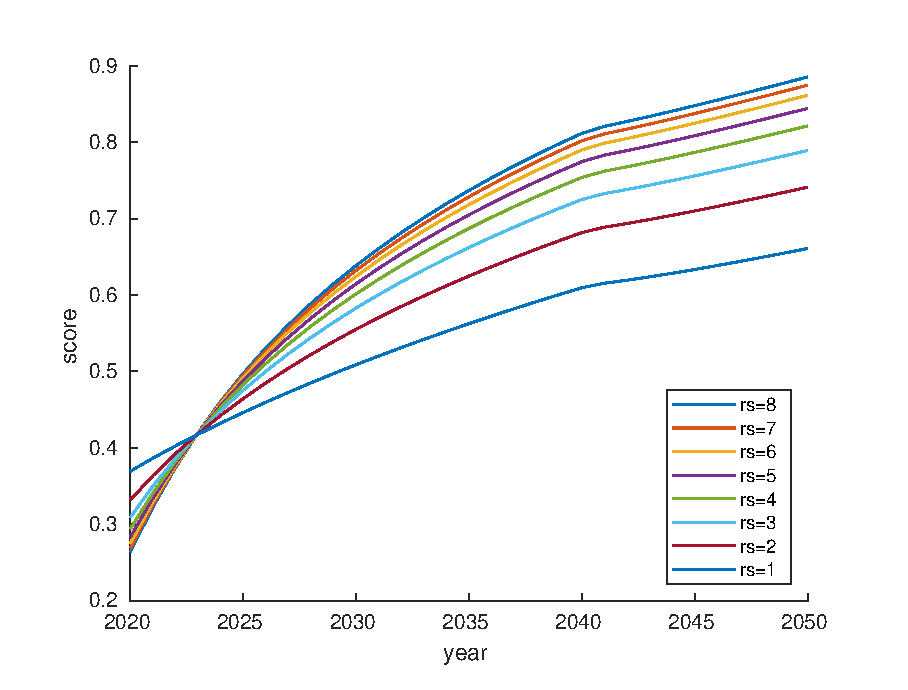
\includegraphics[width = 0.6\textwidth]{figure/sense/sense_AHP.eps}
    \caption{Sensitivity Test for $rs$ by Re-calculating the Corresponding \textit{PFSI}.\label{fig:sense_rs}}
\end{figure}

%%%%%%%%%%%%%%%%%%%%%%%%%%%%%
\section{Strengths and Possible Improvements}
\subsection{Strength}

\begin{itemize}
    \item \textbf{Practicability}: To make our model conform to reality, we divide the food into six groups: cereal. fruit, oil crops, vegetable, dairy, and meat. The model considers all the components of the dietary pyramid.
    \item \textbf{Globality}: We have a macroscopic view of the current food system in the world without taking internal effects into account.
    \item \textbf{Flexibility}: By introducing a variable parameter named policy motivation ($PM$), we can adjust the priorities of efficiency, profitability, sustainability, and equity accordingly. Assigning $PM$ with different possible values (implying that the intensity of policy motivation may vary), our prediction result can be varied to be more flexible.
\end{itemize}

\subsection{Possible Improvements}

\begin{itemize}
    \item \textbf{We do not consider imports and exports}. If for a particular country there is a huge difference between the total amount of food imports and exports, the deviation of our model with reality will increase. 
    \item \textbf{Indicators for our model could be more comprehensive}. In the model of equity, we can add another parameter depicting the matching degree of the dietary structure and the production structure, so that differences in the food distribution within countries can be considered. In addition, in the model of sustainability, more indicators except for greenhouse gas emissions may be added to improve the completeness of the model. The cost of food production may also be included to perfect the model. 
\end{itemize}


\section{Conclusions}

In this paper, we first adopt the logistic model to predict the population growth from 2020 to 2050. Next, we build four models for evaluating efficiency, profitability, equity, and sustainability respectively. We use differential equations, linear programming, and linear fitting to help to find the solutions of our model. Then we propose an index called Prioritized Food System Index ($PFSI$) to denote the emphasis of the food system. In the discussion part, we analyze the benefits and costs for re-optimizing the food system, do case studies on China, the USA, and Ethiopia, and discuss the scalability and adaptability of the model. Finally, we conduct a sensitivity analysis to show the influence of policy motivation on the food system index and discuss strengths as well as improvements for our work.


\bibliographystyle{IEEEtran}
\bibliography{mybib}

% \newpage
\begin{appendices}
\section{Supporting Figures}
\begin{figure}[htbp]
    \centering
    \begin{minipage}[t]{0.48\textwidth}
        \centering
        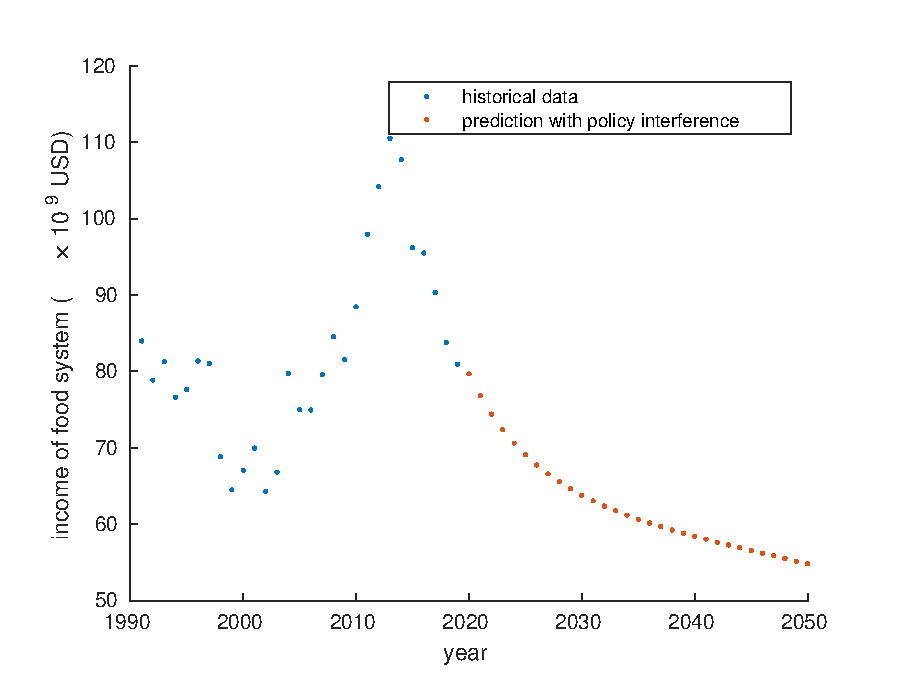
\includegraphics[width=0.7\textwidth]{figure/model/USA/USA_profit.eps}
        \caption{Income of Food System of USA with Policy Interference.}
    \end{minipage}
    \begin{minipage}[t]{0.48\textwidth}
        \centering
        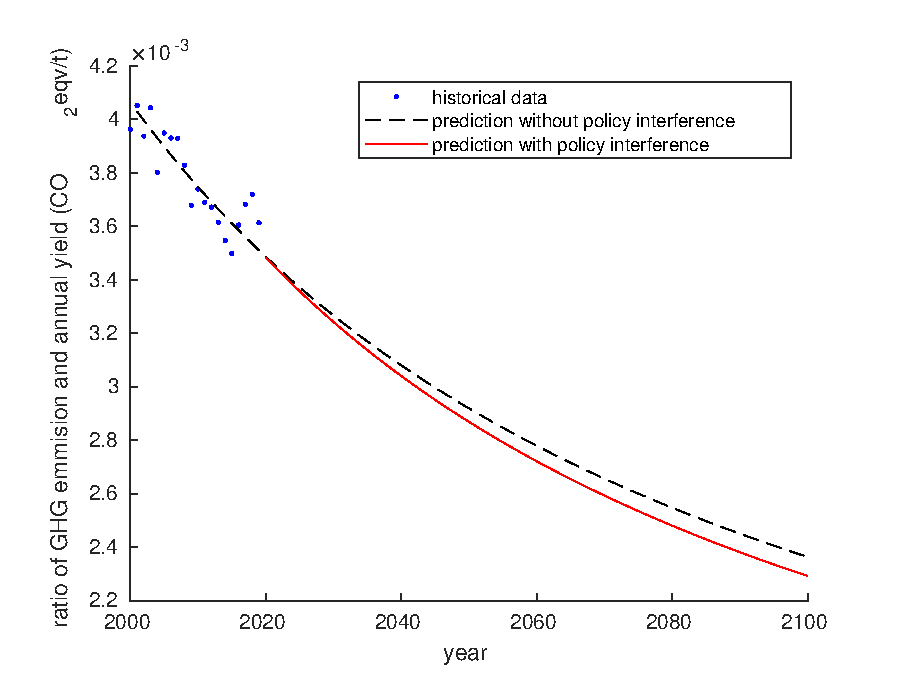
\includegraphics[width=0.7\textwidth]{figure/model/USA/USA_sustainability.eps}
        \caption{Greenhouse Gas Emission per yield of the Food System of USA with Policy Interference.}
    \end{minipage}
\end{figure}
\begin{figure}[htbp]
    \centering
    \begin{minipage}[t]{0.48\textwidth}
        \centering
        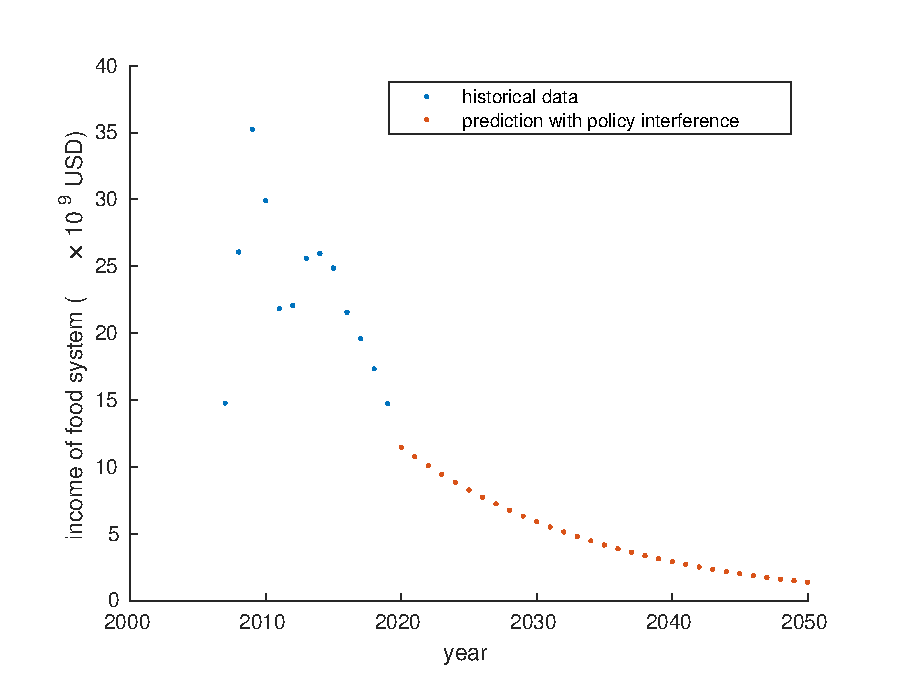
\includegraphics[width=0.7\textwidth]{figure/model/Ethiopia/Ethiopia_profit.eps}
        \caption{Income of Food System of Ethiopia with Policy Interference.}
    \end{minipage}
    \begin{minipage}[t]{0.48\textwidth}
        \centering
        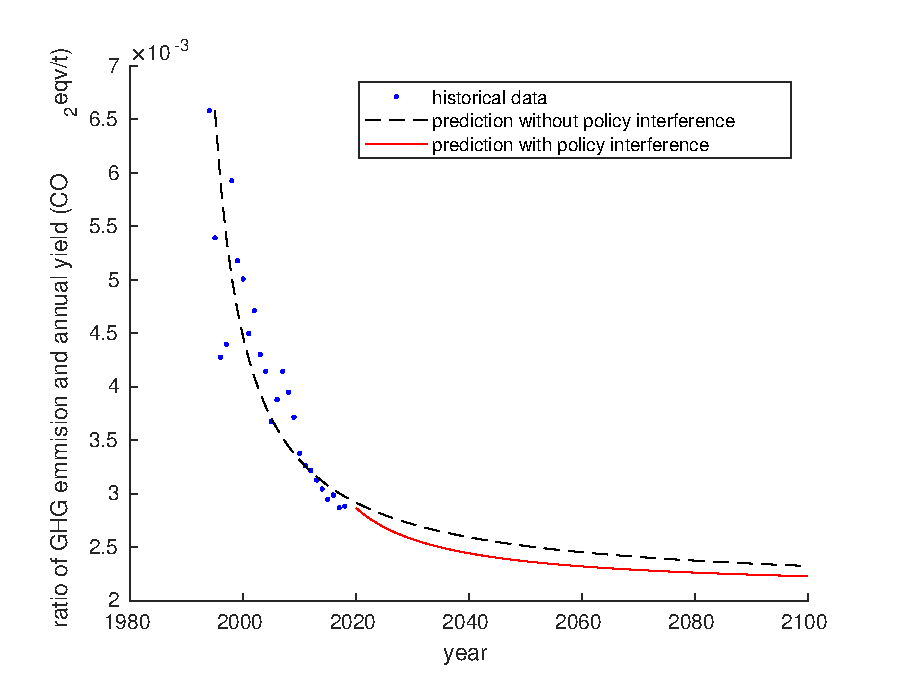
\includegraphics[width=0.7\textwidth]{figure/model/Ethiopia/Ethiopia_sustainability.eps}
        \caption{Greenhouse Gas Emission per yield of the Food System of Ethiopia with Policy Interference.}
    \end{minipage}
\end{figure}
\begin{figure}[htbp]
    \centering
    \begin{minipage}[t]{0.48\textwidth}
        \centering
        \includegraphics[width=0.7\textwidth]{figure/model/USA/USA_GHG_fit.eps}
        \caption{Linear Fit of the Greenhouse Gas Emission of USA.}
    \end{minipage}
    \begin{minipage}[t]{0.48\textwidth}
        \centering
        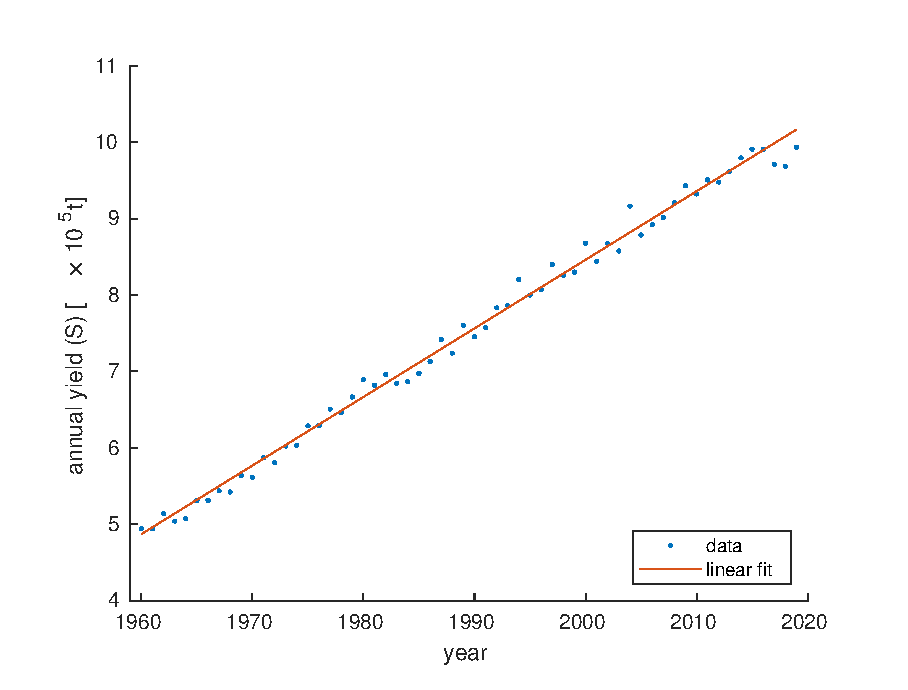
\includegraphics[width=0.7\textwidth]{figure/model/USA/USA_yield_fit.eps}
        \caption{Linear Fit of the Annual Yield of USA.}
    \end{minipage}
\end{figure}
\begin{figure}[htbp]
    \centering
    \begin{minipage}[t]{0.48\textwidth}
        \centering
        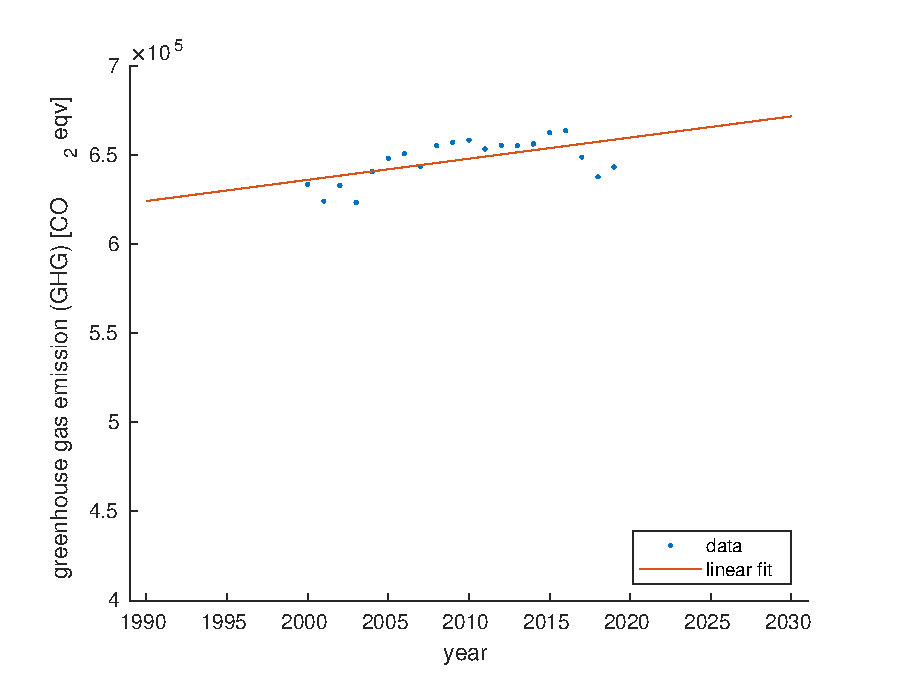
\includegraphics[width=0.7\textwidth]{figure/model/China/China_GHG_fit.eps}
        \caption{Linear Fit of the Greenhouse Gas Emission of China.}
    \end{minipage}
    \begin{minipage}[t]{0.48\textwidth}
        \centering
        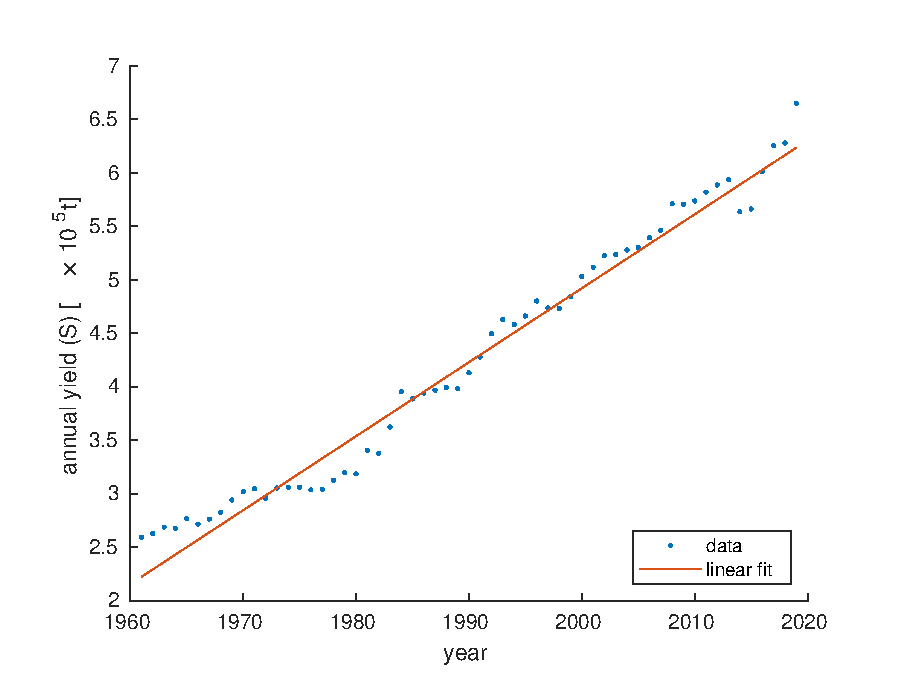
\includegraphics[width=0.7\textwidth]{figure/model/China/China_yield_fit.eps}
        \caption{Linear Fit of the Annual Yield of China.}
    \end{minipage}
\end{figure}
\begin{figure}
    \centering
    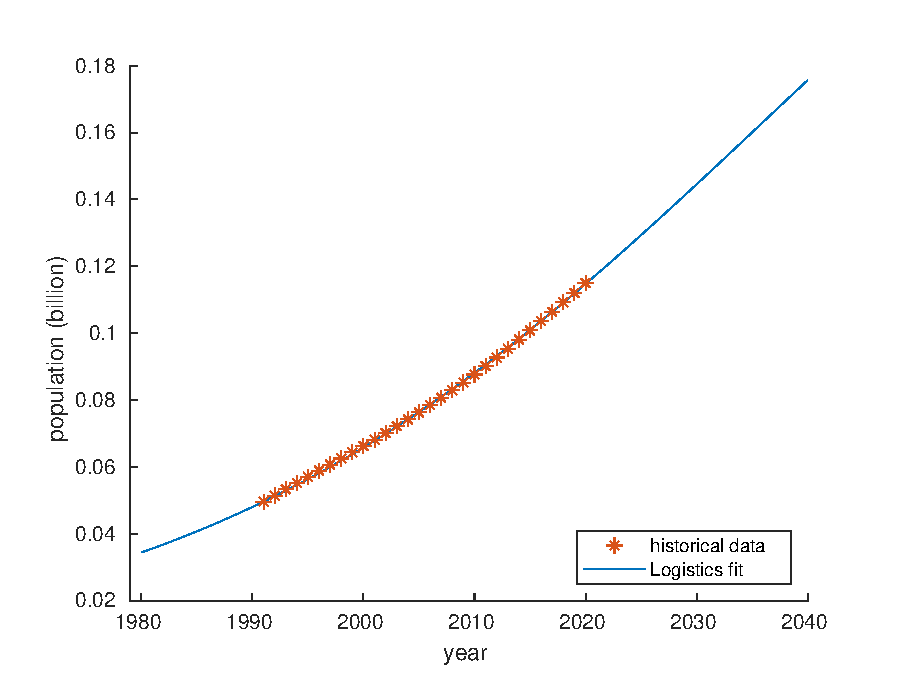
\includegraphics[width = 0.5\textwidth]{figure/model/Ethiopia/Ethiopia_pplt.eps}
    \caption{Logistic Fit of Population of Ethiopia.}
\end{figure}
%     \section{Code Example}
%     %     \lstset{
%     %     basicstyle          =   \sffamily,          % 基本代码风格
%     %     keywordstyle        =   \bfseries,          % 关键字风格
%     %     commentstyle        =   \rmfamily\itshape,  % 注释的风格,斜体
%     %     stringstyle         =   \ttfamily,  % 字符串风格
%     %     flexiblecolumns,                % 别问为什么,加上这个
%     %     numbers             =   left,   % 行号的位置在左边
%     %     showspaces          =   false,  % 是否显示空格,显示了有点乱,所以不现实了
%     %     % numberstyle         =   \zihao{-5}\ttfamily,    % 行号的样式,小五号,tt等宽字体
%     %     showstringspaces    =   false,
%     %     captionpos          =   t,      % 这段代码的名字所呈现的位置,t指的是top上面
%     %     frame               =   lrtb,   % 显示边框
%     % }

%     \vspace{-2em}
%     \lstset{frame=tb,
%         language=Python,
%         aboveskip=3mm,
%         belowskip=3mm,
%         showstringspaces=false,
%         columns=flexible,
%         basicstyle={\small\ttfamily},
%         numbers=none,
%         numberstyle=\tiny\color{gray},
%         keywordstyle=\color{blue},
%         % commentstyle=\color{dkgreen},
%         % stringstyle=\color{mauve},
%         breaklines=true,
%         breakatwhitespace=true,
%         tabsize=3
%     }
%     % \lstdefinestyle{Python}{
%     %     language        =   Python, % 语言选Python
%     %     basicstyle      =   \tt
%     %     % numberstyle     =   \zihao{-5}\ttfamily,
%     %     keywordstyle    =   \color{blue},
%     %     % keywordstyle    =   [2] \color{teal},
%     %     stringstyle     =   \color{magenta},
%     %     commentstyle    =   \color{red}\ttfamily,
%     %     breaklines      =   true,   % 自动换行,建议不要写太长的行
%     %     columns         =   fixed,  % 如果不加这一句,字间距就不固定,很丑,必须加
%     %     basewidth       =   0.5em,
%     % }
%     % \lstinputlisting[title = Grey Forecast]{code/GreyPre.py}
%     \lstinputlisting[title = Moving Entropy Weight Method]{code/EWM.py}
%     \lstinputlisting[title = Grey Forecast]{code/GreyPre.py}


\end{appendices}
\end{document}

